\documentclass[11pt,a4paper]{article}
\usepackage[utf8]{inputenc}
\usepackage[french]{babel}
\usepackage[T1]{fontenc}
\usepackage{amsmath}
\usepackage{amsfonts}
\usepackage{amssymb}
\usepackage{makeidx}
\usepackage{graphicx}

\usepackage{tcolorbox}

\usepackage{lmodern}

\usepackage[left=2cm,right=2cm,top=2cm,bottom=2cm]{geometry}
\author{AMONA Birewa Audrey}
\title{ Tp 06 Sécurité et site administration }
\begin{document}
\maketitle
\tableofcontents
\begin{abstract}
Ce Tp a pour objectif de générer les documents pdf à partir du moteur jinja2 et du template Latex
\end{abstract}
\section{Mise en route}
Nous allons installer les paquet suivant:
\begin{tcolorbox} 
pip install latex\\
pip install jinja2\\
sudo apt install texlive-lang-franch
\end{tcolorbox}
\section{Création du module controlleur et du template}
\begin{enumerate}
\item Créons le dossier \textbf{templating\_ifnti} à la racine de notre projet. Créons le fichier \textbf{controleur.py} dans ce dossier. Ensuite, on édite le fichier comme suit:
	\begin{center}
		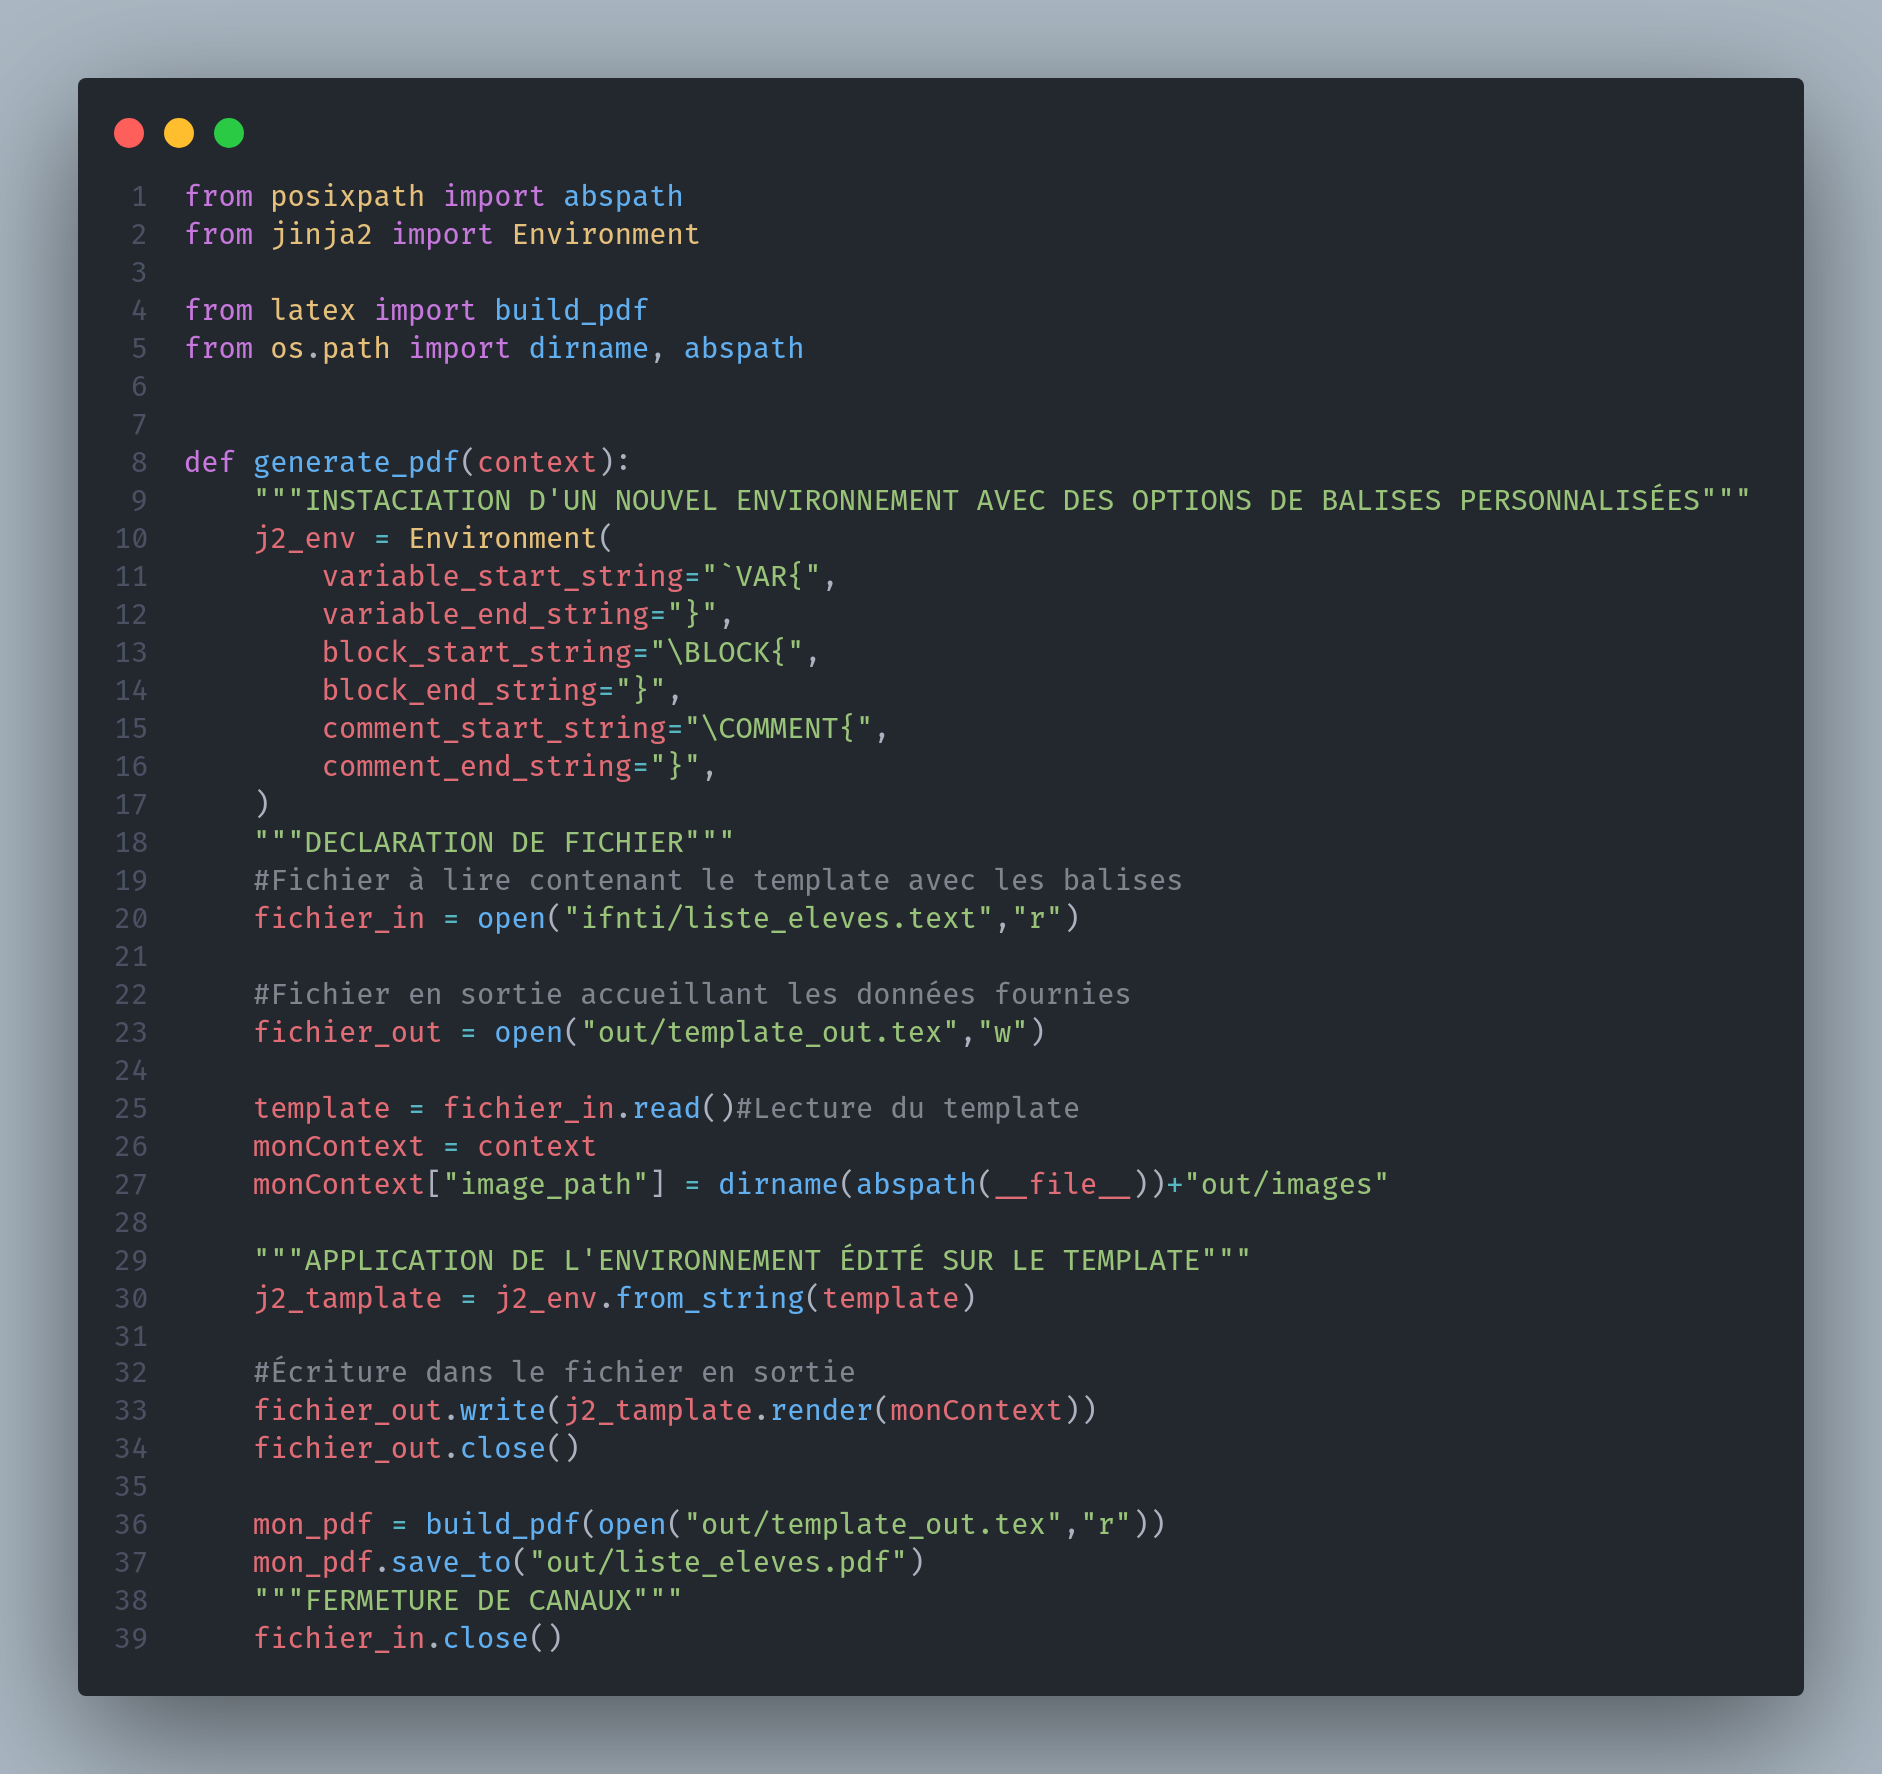
\includegraphics[scale=0.2]{images/code.png}
	\end{center}
Ce code permet de définir des variables d'environnement qui seront utiliser pour injecter des variables ou des structures de controles dans notre fichier de template. Il permet également de définir les fichier templates et de sorties ainsi que le pdf qui sera produit.
\item Créons les dossiers nommés \textbf{ifnti} et \textbf{out}. Créons ensuite les fichiers \textbf{liste\_eleves.tex} dans le dossier \textbf{ifnti}. Puis on y place le code suivant:
\begin{center}
		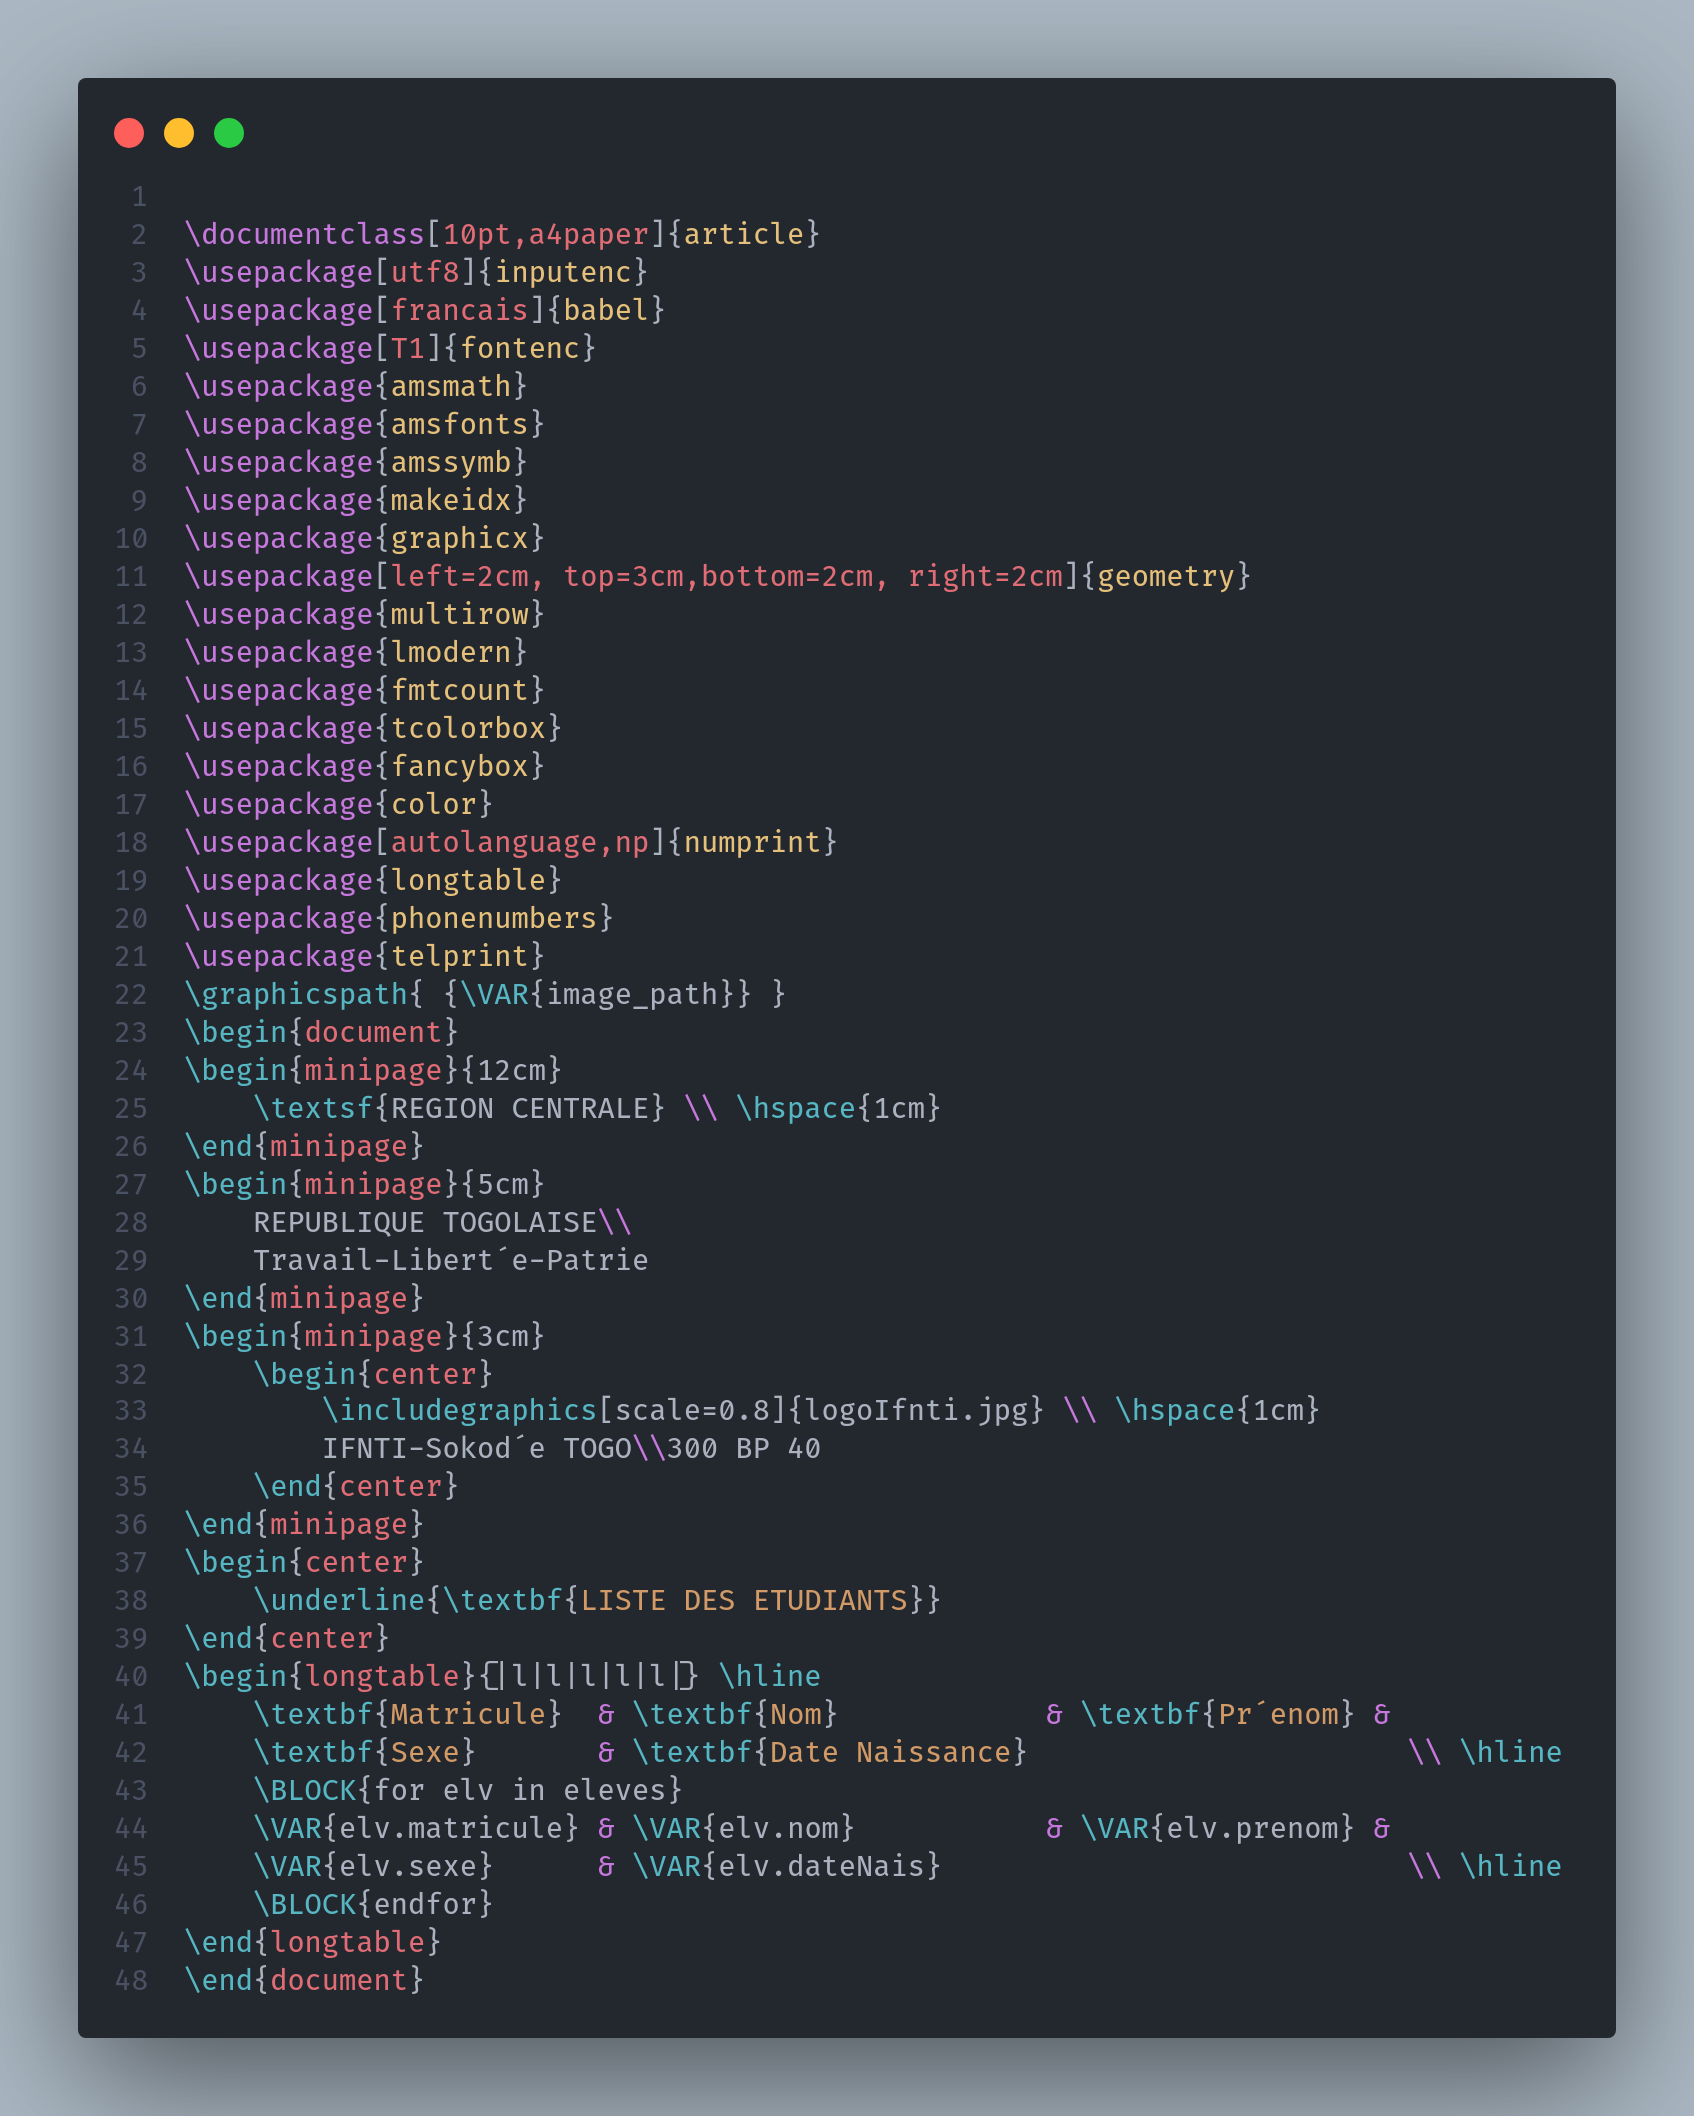
\includegraphics[scale=0.2]{images/tex.png}
	\end{center} Nous allons créer le dossier \textbf{images} dans notre dossie \textbf{out} et y placer le logo de l'ifnti avec le meme nom que celui dans le template.
	\begin{center}
		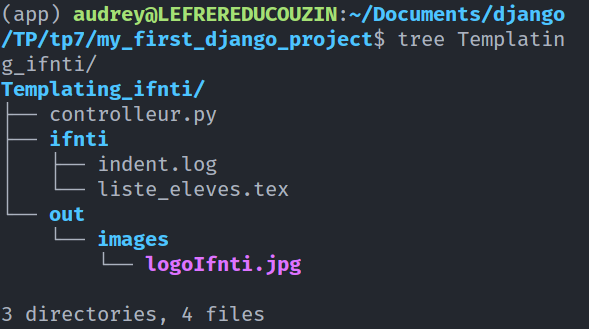
\includegraphics[scale=0.5]{images/arch.png}
	\end{center}
\end{enumerate}
\section{Définition de vues django}
Dans cette section , nous allons définir des vues qui devront retourner des dictionnaires. Ces dictionnaire serviront d'argument à la fonction generate\_pdf()
\begin{enumerate}
	\item Définissons la vue \textbf{listEleves} permettant d'ouvrir un ficher pdf quelconque.
		\begin{center}
		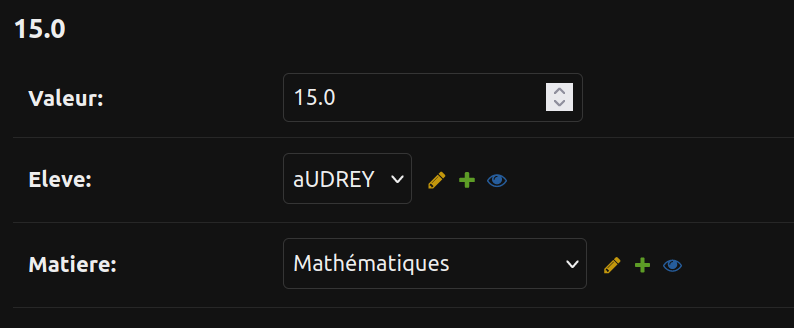
\includegraphics[scale=0.3]{images/test.png}
	\end{center}
			\begin{center}
		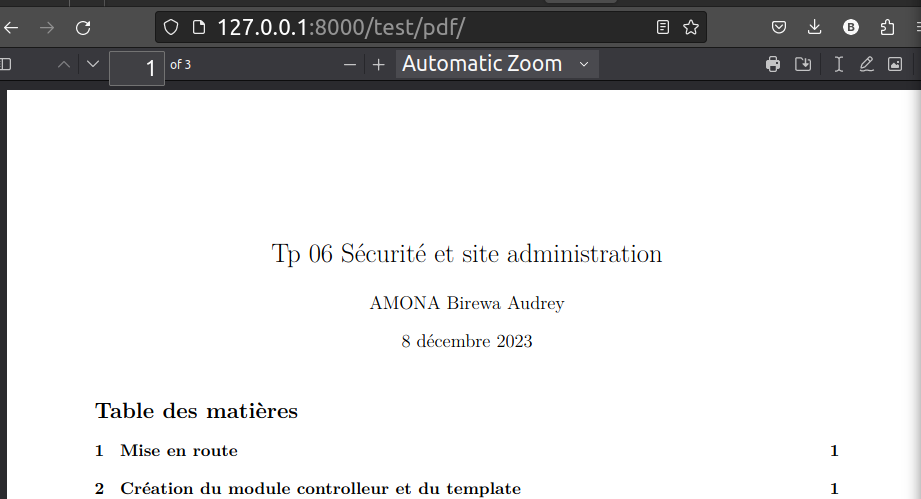
\includegraphics[scale=0.3]{images/pdf.png}
	\end{center}
	\item Nous allons modifier la vue précédente pour générer la liste des élèves
	\begin{center}
		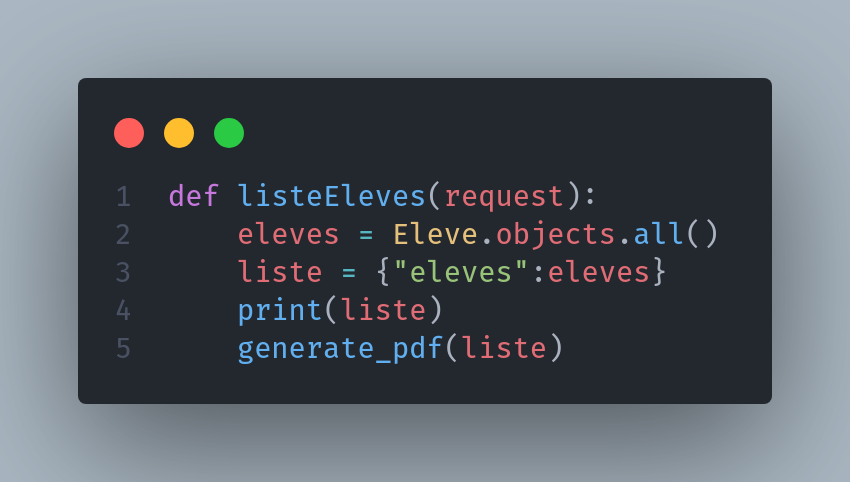
\includegraphics[scale=0.5]{images/gen.png}
	\end{center}
	\begin{center}
		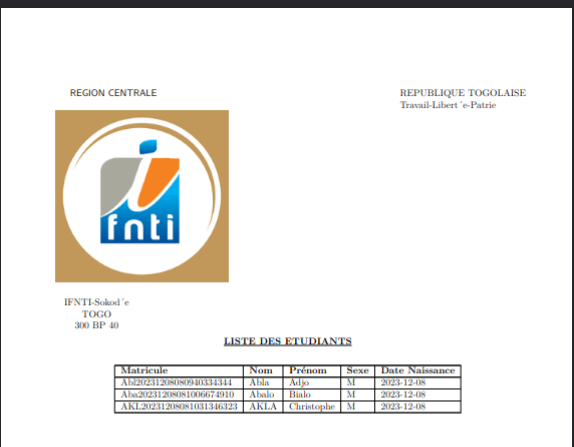
\includegraphics[scale=0.3]{images/pdfout.png}
	\end{center}
	\item Nous allons à présent créer la vue \textbf{liste\_niveauElv} permettant de générer la liste des élèves d'un niveau donné:
		\begin{center}
		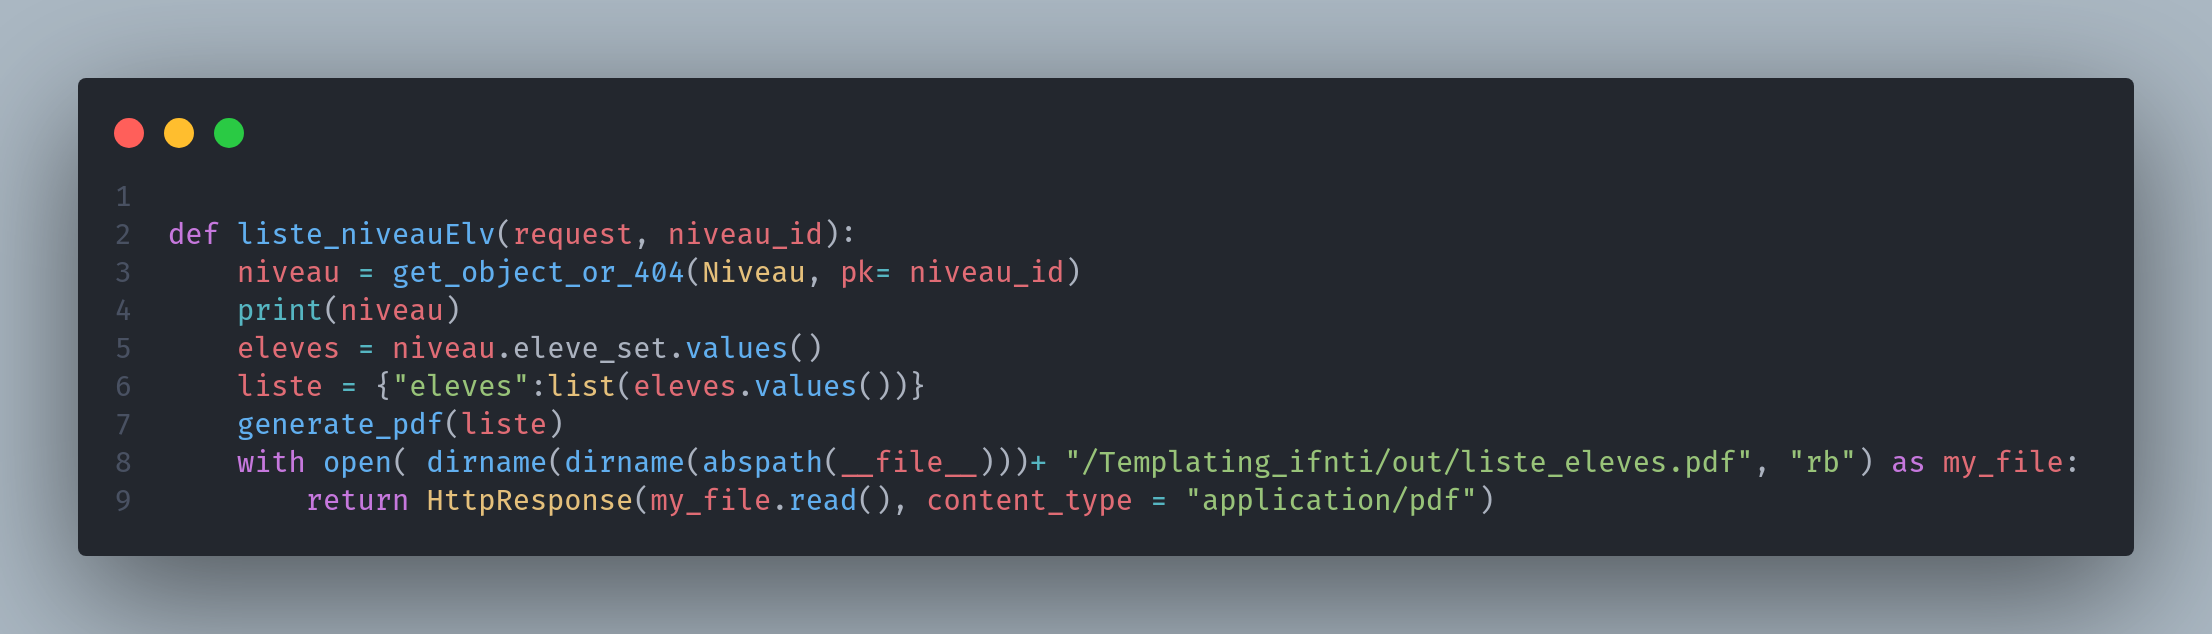
\includegraphics[scale=0.2]{images/gen1.png}
	\end{center}
	\begin{center}
		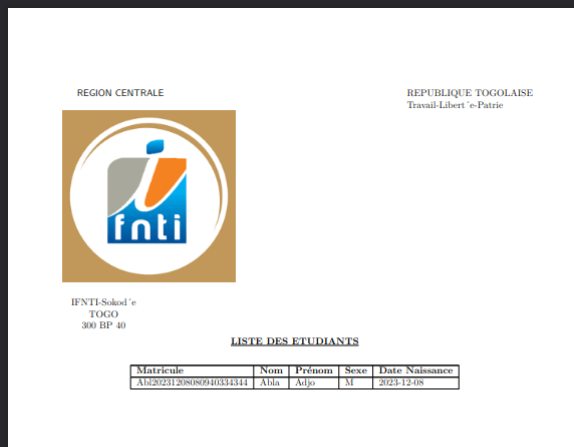
\includegraphics[scale=0.3]{images/pdfout1.png}
	\end{center}
\end{enumerate}
\section{Création de template, controleur et vue}
\end{document}